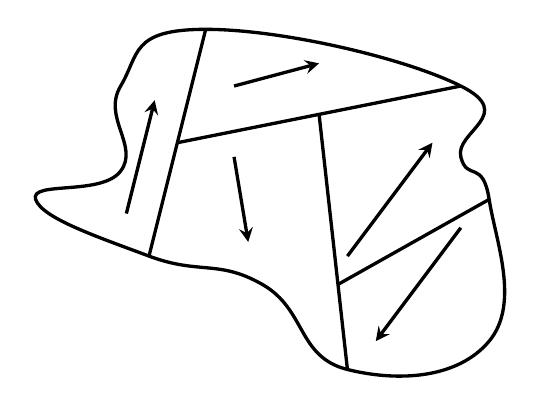
\begin{tikzpicture}[line width = 1.2pt, line join=round,x=0.4cm,y=0.4cm,>=stealth, scale=0.9]
	\coordinate (a) at (0,0);
	\coordinate (b) at (4,-1);
	\coordinate (c) at (7,-4);
	\coordinate (d) at (12,-3);
	\coordinate (e) at (12,2);
	\coordinate (f) at (11,3.5);
	\coordinate (g) at (11,6);
	\coordinate (h) at (2,8);
	\coordinate (i) at (-1,6);
	\coordinate (j) at (-1,3);
	\coordinate (k) at (-4,2);
	% Zwischenpunkte (halbe Strecken meist
	\coordinate (ah) at (1,4);
	\coordinate (ahg) at (6,5);
	% 1/3
	\coordinate (ahgi) at ({6+2/3},-1);
	% Rahmen
	\draw plot [smooth cycle, tension=0.8] coordinates {(a) (b) (c) (d) (e) (f) (g) (h) (i) (j) (k)};
	% Trennlinien
	\draw (a) -- (h);
	\draw (ah) -- (g);
	\draw (ahg) -- (c);
	\draw (ahgi) -- (e);
	% Pfeile
	\draw [->] (-0.8,1.5) -- ++(1,4);
	\draw [->] (3,6) -- ++(3,0.8);
	\draw [->] (3,3.5) -- ++(0.5,-3);
	\draw [->] (7,0) -- ++(3,4);
	\draw [->] (11,1) -- ++(-3,-4);
\end{tikzpicture}